\begin{figure}[t]
  \centering
  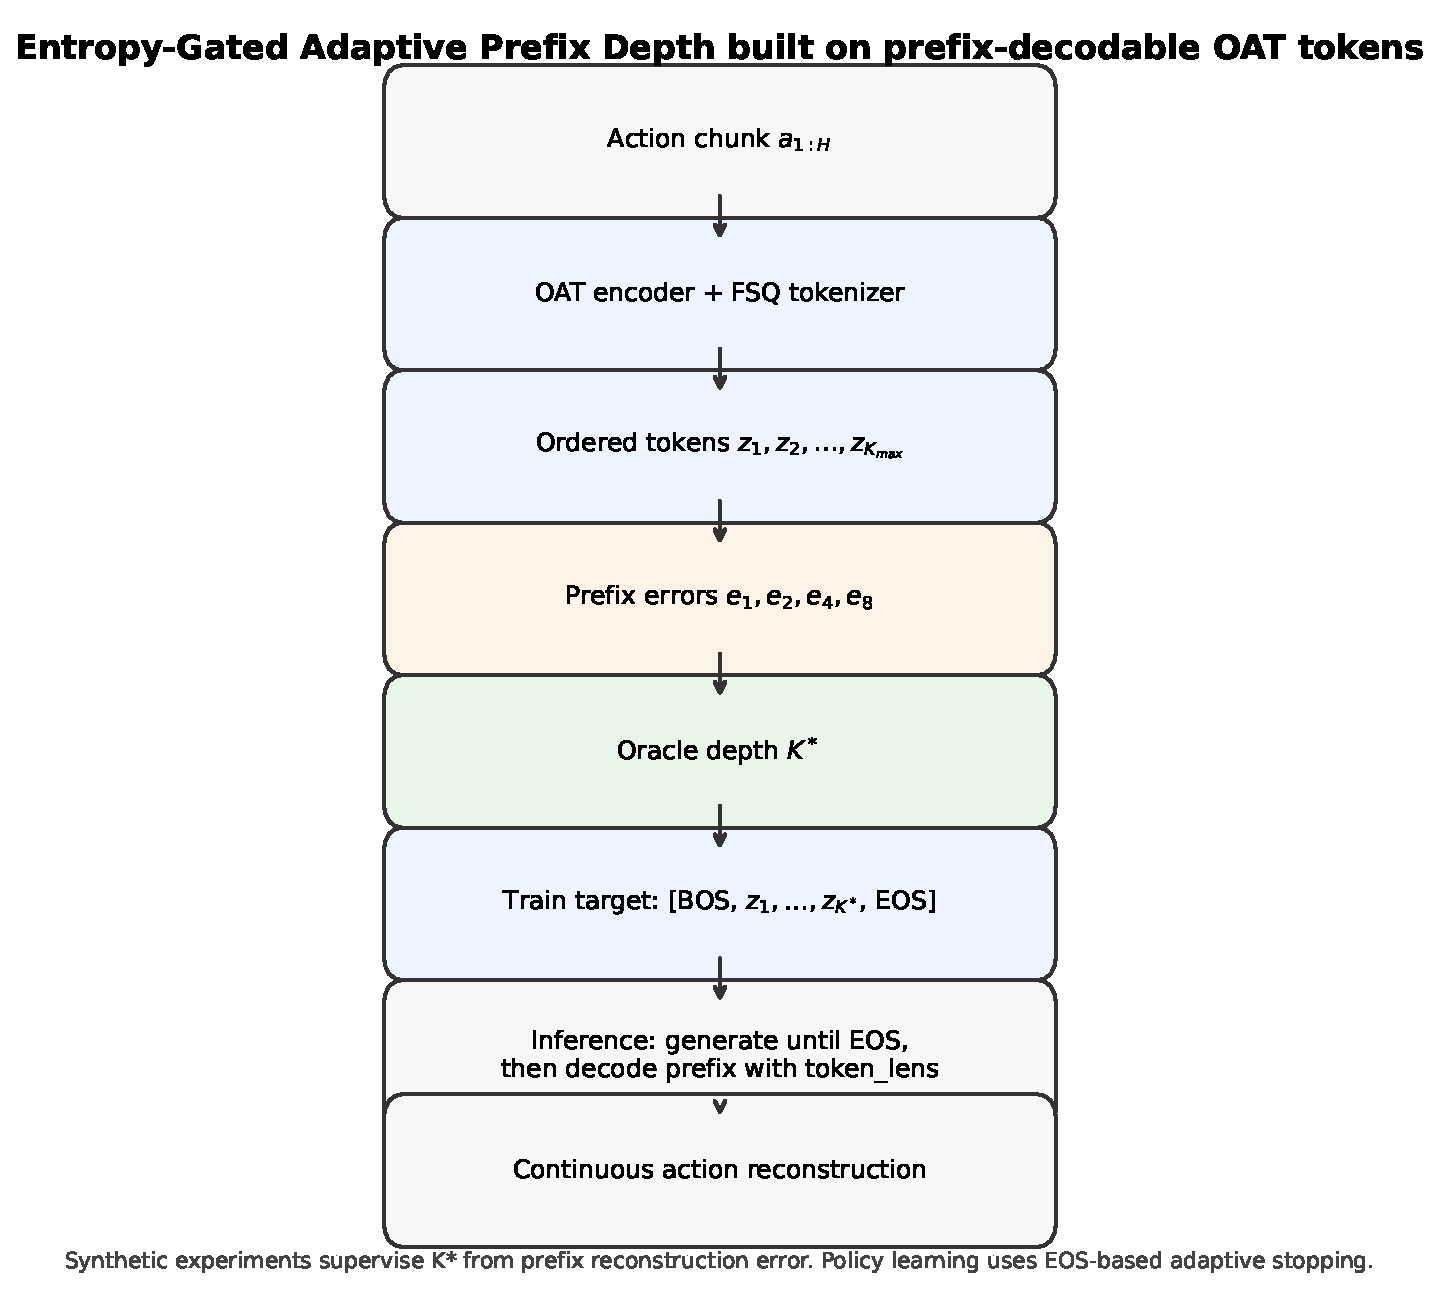
\includegraphics[width=\linewidth]{paper_figures/fig_method_eg_apd_oat.pdf}
  \caption{Method overview of entropy-gated adaptive prefix depth built on ordered, prefix-decodable OAT action tokens. Synthetic experiments supervise the oracle stopping depth $K^*$ from prefix reconstruction error, and policy learning converts adaptive stopping into EOS prediction.}
  \label{fig:fig_method_eg_apd_oat}
\end{figure}

\begin{figure}[t]
  \centering
  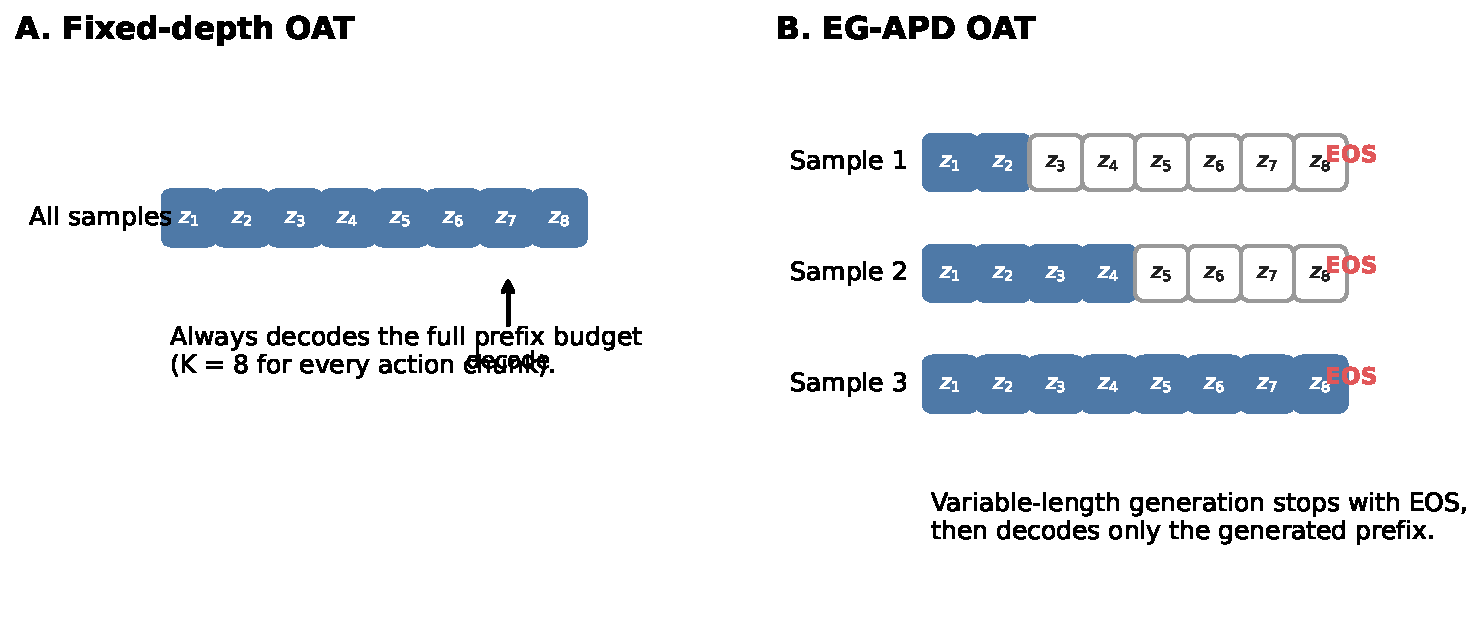
\includegraphics[width=\linewidth]{paper_figures/fig_fixed_vs_adaptive.pdf}
  \caption{Fixed-depth OAT allocates the same token budget to every action chunk, whereas the adaptive variant terminates token generation with EOS after a variable number of ordered action tokens.}
  \label{fig:fig_fixed_vs_adaptive}
\end{figure}

\begin{figure}[t]
  \centering
  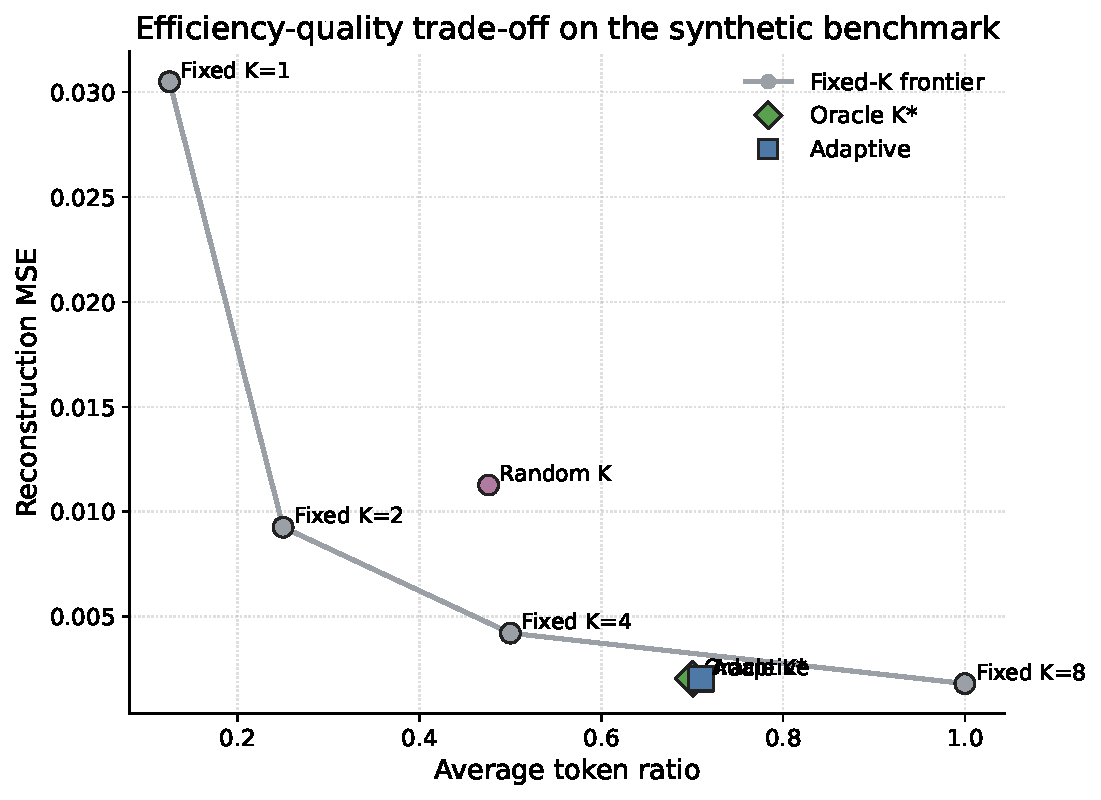
\includegraphics[width=\linewidth]{paper_figures/fig_efficiency_quality_pareto.pdf}
  \caption{Efficiency-quality trade-off on the synthetic benchmark. Fixed-K baselines trace the reconstruction frontier; the adaptive method approaches oracle behavior while reducing token usage relative to full-length decoding.}
  \label{fig:fig_efficiency_quality_pareto}
\end{figure}

\begin{figure}[t]
  \centering
  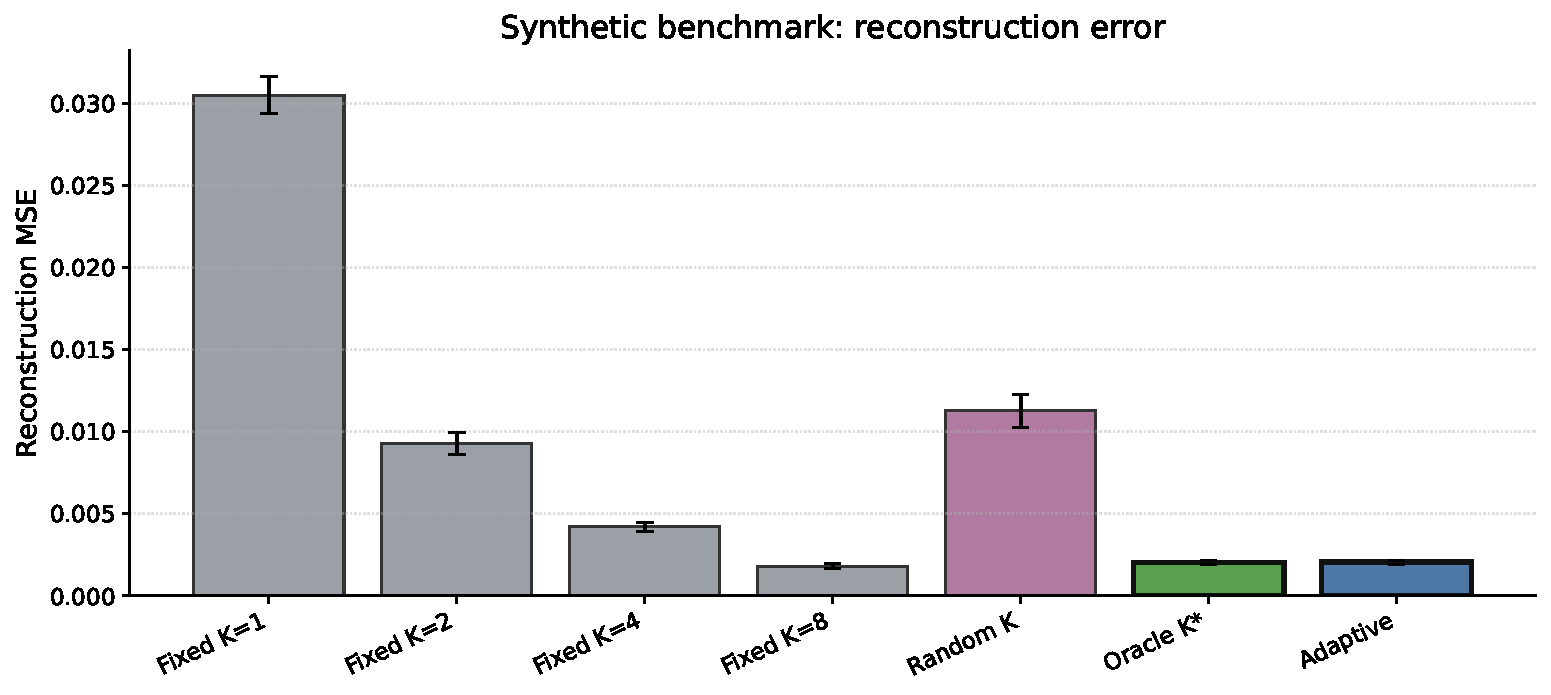
\includegraphics[width=\linewidth]{paper_figures/fig_reconstruction_mse.pdf}
  \caption{Synthetic benchmark reconstruction error across fixed, random, oracle, and adaptive prefix-selection baselines. Error bars show variability across repeated runs.}
  \label{fig:fig_reconstruction_mse}
\end{figure}

\begin{figure}[t]
  \centering
  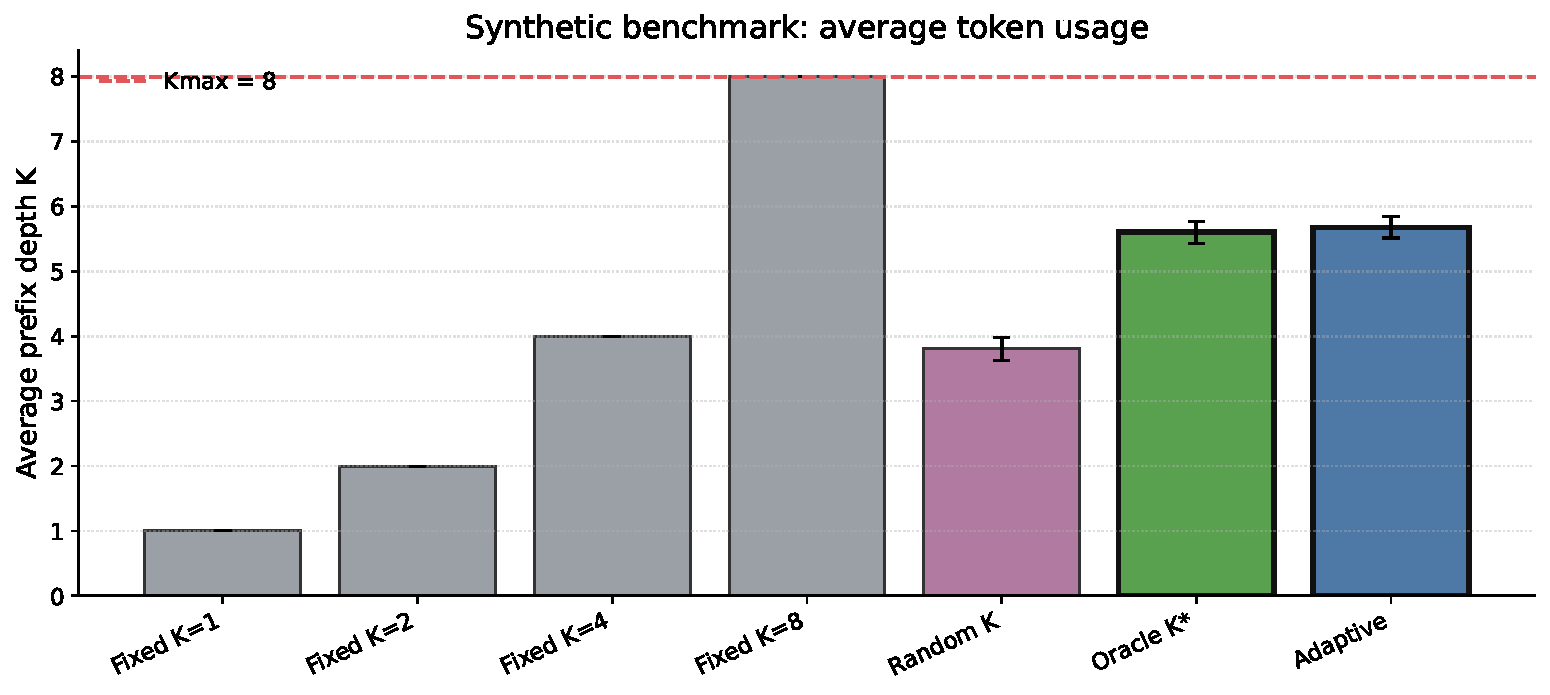
\includegraphics[width=\linewidth]{paper_figures/fig_avg_token_usage.pdf}
  \caption{Average selected prefix depth on the synthetic benchmark. The adaptive method uses fewer than the full $K_{max}=8$ tokens on average.}
  \label{fig:fig_avg_token_usage}
\end{figure}

\begin{figure}[t]
  \centering
  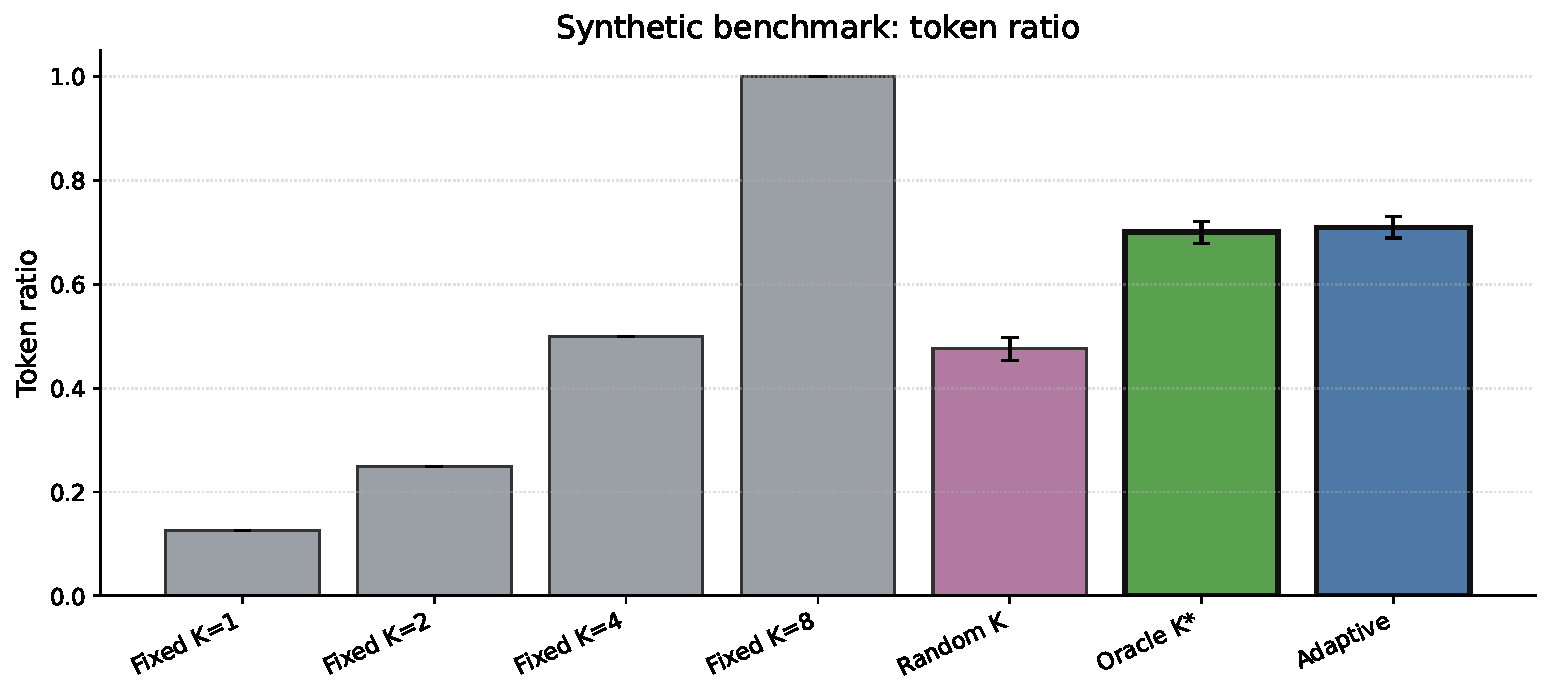
\includegraphics[width=\linewidth]{paper_figures/fig_token_ratio.pdf}
  \caption{Average token ratio relative to the full OAT prefix budget. Adaptive halting reduces average token usage substantially relative to fixed $K=8$ decoding.}
  \label{fig:fig_token_ratio}
\end{figure}

\begin{figure}[t]
  \centering
  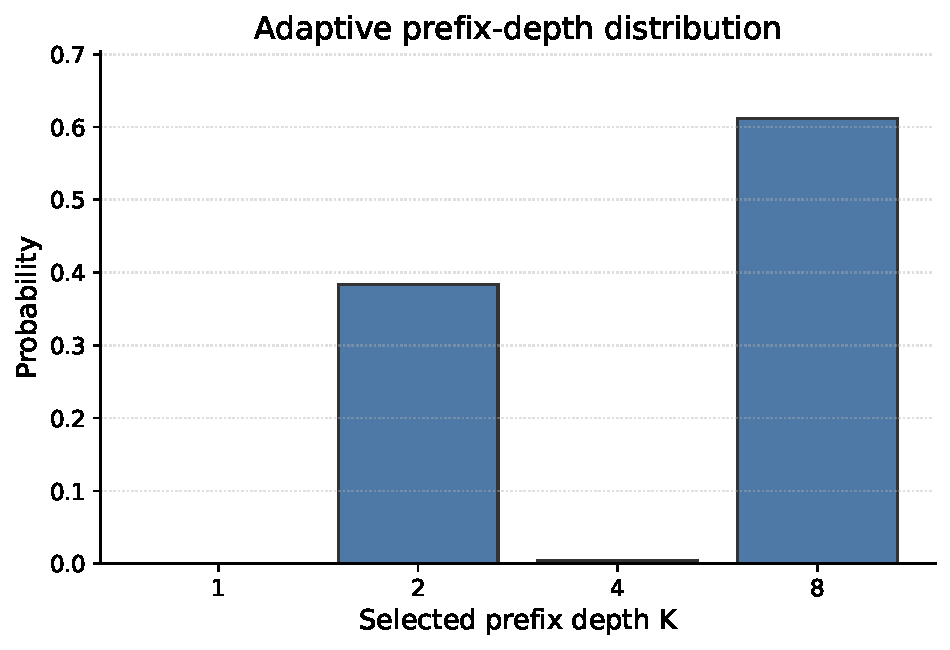
\includegraphics[width=\linewidth]{paper_figures/fig_adaptive_k_distribution.pdf}
  \caption{Distribution of adaptive prefix depths selected on the synthetic benchmark. The learned policy concentrates on a subset of valid ordered-prefix depths rather than using a single fixed budget.}
  \label{fig:fig_adaptive_k_distribution}
\end{figure}

\begin{figure}[t]
  \centering
  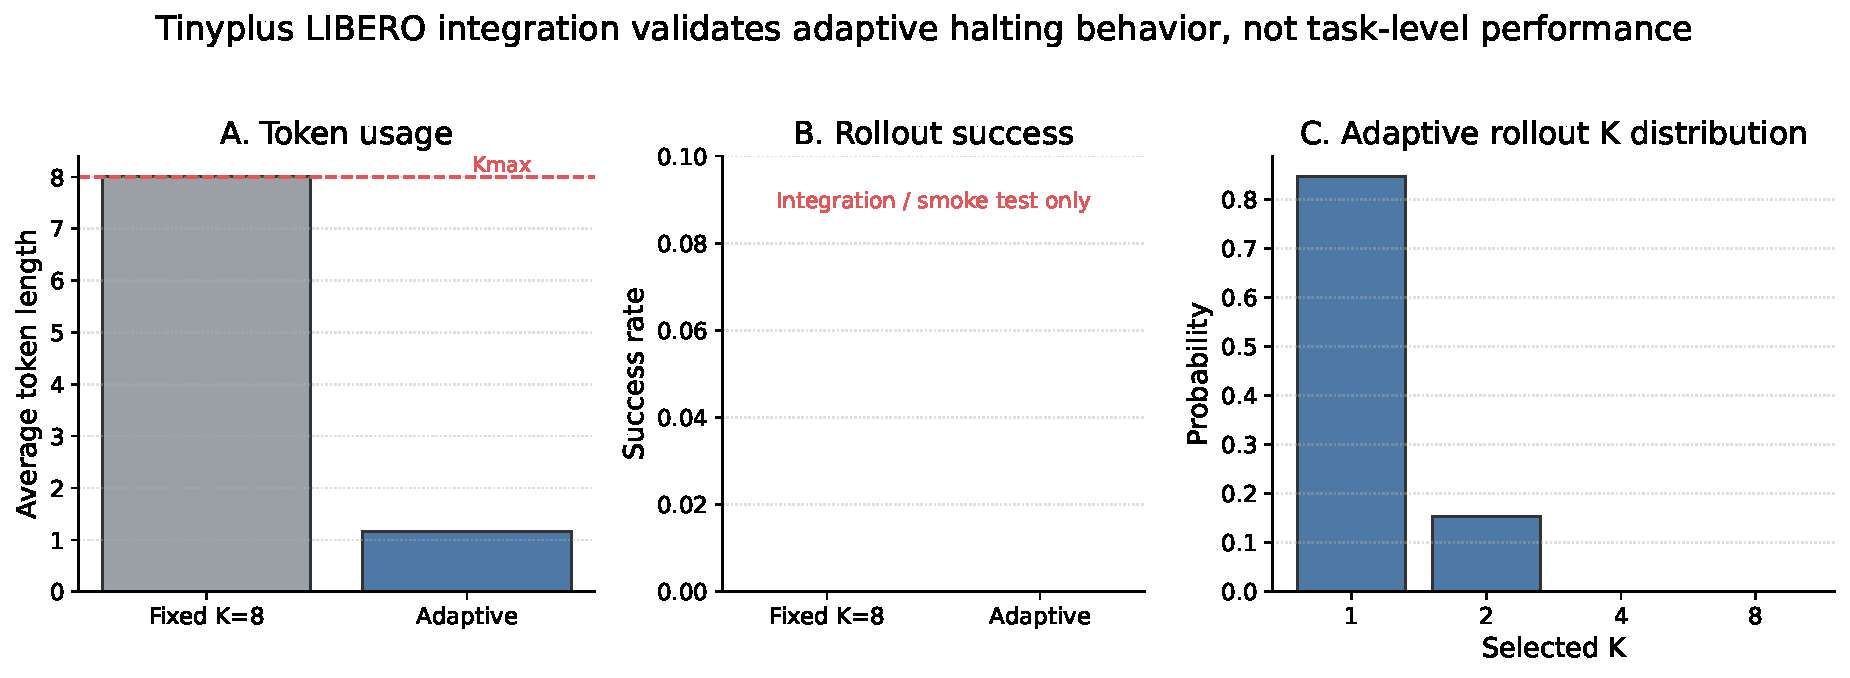
\includegraphics[width=\linewidth]{paper_figures/fig_libero_tinyplus_integration.pdf}
  \caption{Tinyplus LIBERO rollout results. Adaptive halting changes token usage and prefix-length behavior in the real simulator stack, but both methods remain at zero task success; this figure is integration validation rather than benchmark evidence.}
  \label{fig:fig_libero_tinyplus_integration}
\end{figure}

\begin{figure}[t]
  \centering
  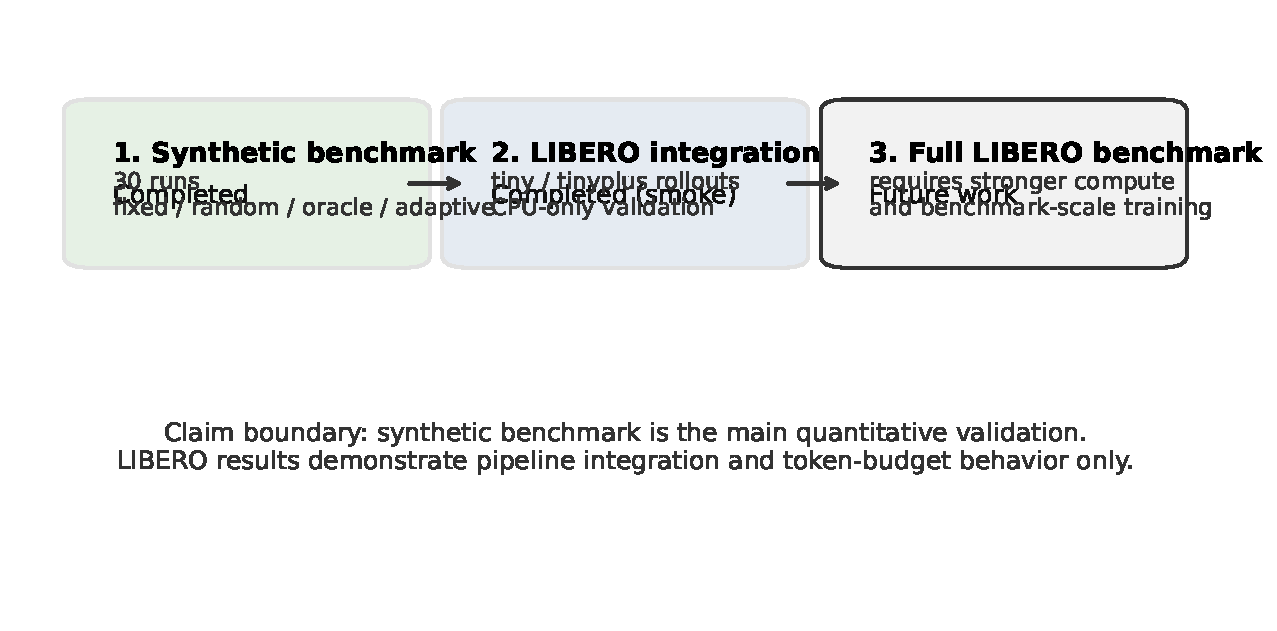
\includegraphics[width=\linewidth]{paper_figures/fig_evaluation_pipeline_status.pdf}
  \caption{Evaluation status summary. Synthetic experiments provide the main quantitative evidence, while LIBERO results currently validate integration and adaptive stopping behavior under limited CPU-only training.}
  \label{fig:fig_evaluation_pipeline_status}
\end{figure}
